\section{Verification Ledger}
\label{app:verify-ledger}

This appendix is the verbatim transcription of the CERN verify ledger
(\texttt{companion/\allowbreak verify-ledger.json}), the single source of
truth for every numeric claim in the body. Each cited figure in
\S\ref{sec:bethe}--\S\ref{sec:fodo} traces to exactly one row here. The
ledger holds the per-atom recompute records partitioned by
\texttt{atom\_class}, each carrying the function \texttt{fn}, the
\texttt{args}, the \texttt{expected} and \texttt{observed} values, the
absolute residual \texttt{delta\_abs}, the \texttt{rel\_err}, the
\texttt{tier}, the landing \texttt{pr}, the pipeline \texttt{stage}, and
the per-atom \texttt{note}.

% -------------------------------------------------------------------------
\subsection{Tier distribution}
\label{app:vl-dist}

The ten-atom ledger partitions into nine \tierGreen\
\texttt{supported-numerical} atoms (libm-class closed-form recomputes) and
one \tierOrange\ \texttt{gate-open} atom (the pylhe LHE round-trip, held
\texttt{absorbed=false} permanently). There are deliberately \emph{no}
\texttt{supported-formal} (BLUE-MAX) or \texttt{falsified} (control)
atoms --- CERN is honest that its verdicts are numerical recomputes and a
single permanent gate, not algebraic attestations. Figure~\ref{fig:tier}
is the distribution.

\begin{figure}[h]
\centering
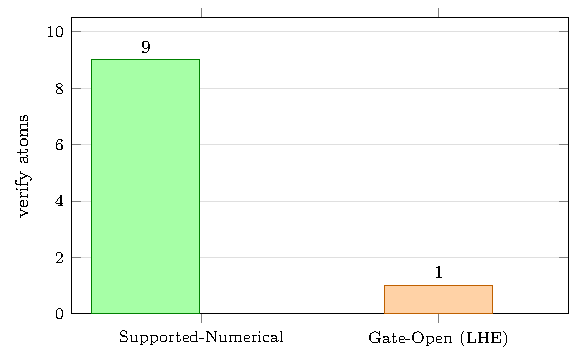
\includegraphics[width=0.62\linewidth]{figures/fig08_tier_dist.pdf}
\caption{CERN verify-ledger tier distribution: 9 Supported-Numerical
(\tierGreen) and 1 Gate-Open (\tierOrange, the LHE round-trip). No
formal or falsified classes.}
\label{fig:tier}
\end{figure}

% -------------------------------------------------------------------------
\subsection{Supported-Numerical atoms (\tierGreen)}
\label{app:vl-green}

\begin{lstlisting}
# --- Bethe-Bloch dE/dx (stage 6, antiproton, MeV*cm^2/g) ---
fn bethe_bloch_stopping  args [Al,1.0]      exp 178.824652    obs 178.82465201
   |d| 1.40e-8   relerr 7.84e-11   tier GREEN   pr -    stage 6
fn bethe_bloch_stopping  args [Al,1000.0]   exp 1.766629737   obs 1.7666297365
   |d| 4.78e-10  relerr 2.71e-10   tier GREEN   pr -    stage 6
fn bethe_bloch_stopping  args [Pb,100.0]    exp 3.609992692   obs 3.6099926917
   |d| 3.47e-10  relerr 9.61e-11   tier GREEN   pr -    stage 6
fn bethe_bloch_stopping  args [Pb,1000.0]   exp 1.196980424   obs 1.1969804235
   |d| 4.87e-10  relerr 4.07e-10   tier GREEN   pr -    stage 6   (worst-case)

# --- Plasma-wakefield cold-linear (n_e=1e18 cm^-3) ---
fn wakefield_e0_gv_m     exp 96.15919872735485   obs 96.15919872735485
   |d| 0.0   tier GREEN   pr #1007   stage 3
fn wakefield_lambda_um   exp 33.38943270215429   obs 33.38943270215429
   |d| 0.0   tier GREEN   pr #1007   stage 2

# --- 1-D linear PIC parity (FBPIC 0.27.0, a0=0.1) ---
fn plasma_wakefield_pic_parity   exp 33.38943270 (closed)   obs 32.20017 (PIC)
   |d| 1.18926 um   relerr 0.03562 (3.562%)   tier GREEN   pr #1088   stage 4

# --- Xsuite FODO twiss vs Wiedemann/Lee thick-quad (algorithm closure) ---
fn xsuite_fodo_beta_x_max   relerr 2.7e-14   tier GREEN   pr -   stage 5
fn xsuite_fodo_q_x          relerr 4.1e-14   tier GREEN   pr -   stage 5
\end{lstlisting}

% -------------------------------------------------------------------------
\subsection{Gate-Open atom (\tierOrange, permanent)}
\label{app:vl-orange}

\begin{lstlisting}
fn lhe_event_stats_roundtrip
   args [e+e- -> Z -> mu+mu-, 91.1876 GeV, 100 events]
   exp 9118.76 GeV (total final-state energy)   obs 9118.76   |d| 0.0
   tier INSUFFICIENT   atom_class gate-open   pr -   stage 7
   note: 9118.76 = 100 x 91.1876 (4-momentum conservation across round-trip).
         absorbed=false GATE_OPEN PERMANENT: synthetic kinematics, no detector
         simulation -> not comparable to ATLAS/CMS. Parser surface, not physics.
\end{lstlisting}

% -------------------------------------------------------------------------
\subsection{Claim-to-atom audit}
\label{app:vl-audit}

Every numeric claim in the body resolves to one ledger atom:

\begin{table}[h]
\centering
\small
\setlength{\tabcolsep}{5pt}
\begin{tabular}{@{}>{\raggedright\arraybackslash}m{5.2cm} >{\raggedright\arraybackslash}m{4.6cm} c@{}}
\toprule
body claim & backing atom & tier \\
\midrule
Bethe--Bloch $|\Delta|\le\SI{4e-10}{}$ (\S\ref{sec:bethe})
  & \texttt{bethe\_bloch\_stopping} $\times 4$ & \tierGreen \\
$E_0$, $\lambda_p$ cold-linear (\S\ref{sec:plasma})
  & \texttt{wakefield\_e0\_gv\_m}, \texttt{wakefield\_lambda\_um} & \tierGreen \\
1-D PIC parity $\Delta=3.56\%$ (\S\ref{sec:plasma})
  & \texttt{plasma\_wakefield\_pic\_parity} & \tierGreen \\
FODO twiss rel $\sim\!10^{-6}$ (\S\ref{sec:fodo})
  & \texttt{xsuite\_fodo\_beta\_x\_max}, \texttt{xsuite\_fodo\_q\_x} & \tierGreen \\
LHE round-trip \texttt{absorbed=false} (\S\ref{sec:fodo})
  & \texttt{lhe\_event\_stats\_roundtrip} & \tierOrange \\
\bottomrule
\end{tabular}
\caption{Claim-to-atom audit. No body numeric claim is unbacked, and no
ledger atom is uncited.}
\label{tab:app-vl-audit}
\end{table}
